\documentclass[25pt, a0paper,portrait]{tikzposter} %orientation options: portrait, landscape
% \geometry{paperwidth=84.1cm,paperheight=118.9cm}
\geometry{paperwidth=60cm,paperheight=120cm}
\makeatletter
\setlength{\TP@visibletextwidth}{\textwidth-2\TP@innermargin}
\setlength{\TP@visibletextheight}{\textheight-2\TP@innermargin}
\makeatother
\usepackage[utf8]{inputenc}
\usepackage{tikz}
\usepackage{graphicx}
\usepackage{enumitem}

\usetheme{Board} % Options: Default, Simple, Basic, Rays, Wave, Envelope, Board, Autumn, Desert
\tikzposterlatexaffectionproofoff%右下角自带的LaTeX logo

%交大蓝
\definecolor{tdliblue}{RGB}{0,64,152}
\colorlet{backgroundcolor}{tdliblue} % 设置背景颜色为交大蓝
\colorlet{blocktitlefgcolor}{tdliblue}

%%%title page
\newcommand{\mytitle}{Searching for TeV halos millisecond pulsars with stacking analysis}
\author{Hongfei Zhang$^1$, Hao Zhou$^1$, Yu Luo$^1$}
\institute{$^1$Tsung-Dao Lee Institute, Shanghai Jiao Tong University}

%%%title的内容 主要去调\titleposright以及后面的
\definetitlestyle{mytitlestyle}{
        width=50cm, roundedcorners=20, innersep=0pt,
	titletotopverticalspace=2cm, titletoblockverticalspace=2cm,
}{
	\begin{scope}[line width=\titlelinewidth, rounded corners=\titleroundedcorners]
		\draw[color=lightgray, fill=titlebgcolor]
		(\titleposleft-4cm,\titleposbottom) rectangle (\titleposright-4cm,\titlepostop);
	\end{scope}
        \node[anchor=south west] at (\titleposleft-3.5cm,\titleposbottom+0.5cm) {
\includegraphics[width=8cm]{initial_pic/sjtu1.png}}; % 交大蓝图片
}

\title{\mytitle}
\usetitlestyle{mytitlestyle}

%%title的框
\makeatletter
\renewcommand\TP@maketitle{%
	\hspace*{-1cm}
	\begin{minipage}{0.2\linewidth}
		\centering
		\vspace*{1em}
		\hspace*{-5cm}
		\@titlegraphic
		\vspace*{0.5em}
	\end{minipage}%
	\hspace{-4cm}
	\begin{minipage}{40cm}%%%控制标题长度
		\raggedright
		\color{titlefgcolor}
		\vspace*{1em}
		{\bfseries \Huge  \mytitle\par}
		\vspace*{1em}
		{\LARGE \@author}\par
		\vspace*{0.5em}
		{\Large \@institute}
	\end{minipage}%
	\vspace{0.5em}
}
\makeatother
% \usetitlestyle{mytitlestyle}

%import necessary packages
\usepackage{blindtext}%生成随机文本
\usepackage{graphicx}
\usepackage{caption}
\usepackage{subcaption}
\usepackage{comment}
\usepackage{amsmath,amssymb}
\usepackage{slashed}

\begin{document}

\maketitle

% %%LHAASO logo
\node[anchor=east, xshift = -8cm,yshift=-1.5cm] at (TP@title.east) {
\includegraphics[width=10cm]{fig/LHAASO1.png}};

% %%contact info
\node[anchor=north west] at (21cm,57.5cm) {
\includegraphics[width=8cm]{fig/ContactQR.jpg}};

%%%%%%%%%%%%%%%%%%%%%%%%%%%%%%%%%%%%%%%%

\begin{columns}

    \column{0.5}%set width of first column

	 \block{1. Introduction}{
          \begin{itemize}
            \item TeV halos are extended emission regions surrounding pulsars. They are believed to originate from relativistic electrons injected by the pulsar, which radiate TeV photons via inverse Compton scattering in regions of locally suppressed diffusion. 
            \item While most confirmed TeV halos are associated with middle-aged pulsars, it has been proposed that millisecond pulsars (MSPs) could similarly serve as sources of TeV gamma rays.
          \end{itemize}
	}
    
    \block{2. Methods}{
        \begin{itemize}[itemsep=30pt]
            % \item The Large High Altitude Air Shower Observatory (LHAASO) studies high-energy gamma rays and cosmic rays. It comprises three detector arrays: the Water Cherenkov Detector Array (WCDA), the Kilometer Square Array (KM2A), and the Wide Field-of-view Cherenkov Telescope Array (WFCTA). 
            \item This work uses WCDA data from March 5, 2021, to July 31, 2024. 
            \item We selected millisecond pulsars (MSPs) from the ATNF Pulsar Catalogue, applying the following criteria:
        \end{itemize}

        \begin{enumerate}
            \item Period $\mathrm{p_0<=0.01s}$
            \item Spin-down flux $\dot{\mathrm{E}} \mathrm{/D^2>=10^{34}erg/s/kpc^2} $
            \item Declination $\mathrm{ \delta<=70^\circ \ and \ \delta>=-10^\circ }$
            \item To avoid contamination from galactic diffuse emission, we select a conservative galactic latitude range:
            
            $\mathrm{ b>=10^\circ \ or \ b<=-10^\circ }$
            \item Distances to TeVCat sources should be larger than $\mathrm{ \sigma = n * \sqrt{ R_{TeV}^2+PSF^2} }$, where $\mathrm{ n=3 }$, $\mathrm{R_{TeV}}$ is the size of the source recorded in TeVCat, $\mathrm{ PSF=0.5^\circ }$, which corresponds angular resolution of the detector
            \item For extremely large sources, we mask those regions: 
                \begin{itemize}
                    \item Cygnus cocoon($\mathrm{ RA=306.9^\circ,Dec=41.32^\circ,\sigma=6^\circ }$)
                    \item Geminga($\mathrm{ RA=98.5^\circ,Dec=17.76^\circ,\sigma=8^\circ }$)
                    \item Monogem($\mathrm{ RA=104.95^\circ,Dec=14.24^\circ,\sigma=8^\circ }$)
                \end{itemize}
        \end{enumerate}

        \begin{center}
            \begin{minipage}{25cm}
                \centering
                \begin{tikzpicture}
                    \node[inner sep=0pt] (image) at (0,0) {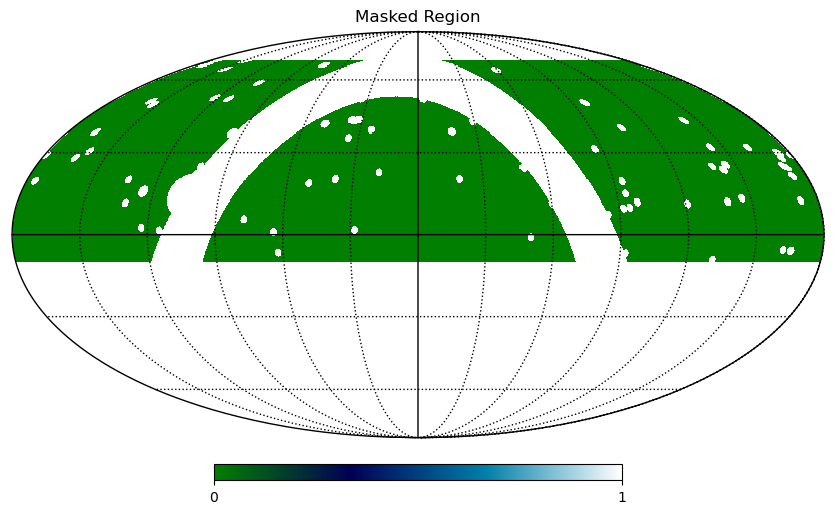
\includegraphics[width=25cm]{fig/sample_space.png}};
                    \node[rotate=45, font=\fontsize{80}{100}\selectfont, color=gray!50, opacity=0.7] at (image.center) {Preliminary};
                \end{tikzpicture}
            \end{minipage}
            
            \begin{minipage}{25cm}
                \centering 
                Fig 1: Schematic of the masked and acceptable areas in equatorial coordinates. White regions are masked during searching MSPs, while green regions are acceptable.
            \end{minipage}
        \end{center}
        \begin{itemize}[itemsep=10pt]
            \item 26 MSPs meet the criteria. Two models were employed: point source model and extended source model. 
            
            \item In extended source model, each source is assumed to be a uniform disk with a radius $\mathrm{ R_{src} = R_{phy}/d }$, where $\mathrm{ R_{phy} }$ is the physical size of the source, which is fixed at 10 pc, d is the distance from the ATNF Pulsar Catalogue, the fifth selection criterion was modified to $\mathrm{ \sigma = n * \sqrt{ R_{src}^2+R_{TeV}^2+PSF^2} }$, thus only 24 MSPs meet the conditions.
        
            \item energy spectrum is weighted power-law: 
                \begin{equation}
                    \mathrm{ \frac{dN}{dE} = F_0 w \left( \frac{E}{E_{piv}} \right)^{\alpha} }
                \end{equation}
                $\mathrm{ E_{piv} }$ is 3 TeV, $ \mathrm{ w = } \dot{ \mathrm{E} } \mathrm{ /D^2 / (10^{34} erg/s/kpc^2) }$.
        
            \item The spectral index $\alpha$ and the normalization $\mathrm{ F_0 }$ were sampled over reasonable ranges. For each combination of $\alpha$ and $\mathrm{ F_0 }$, the test statistic (TS) was calculated using equation:
            \begin{equation}
                \mathrm{TS} = 2\ln{ \frac{ \mathcal{L}_1(\mathrm{ \alpha, F_0 }) }{ \mathcal{L}_0 } }
            \end{equation}
        \end{itemize}
    }
    
    \column{0.5}%set width of second column
    \block{3. Conclusion}{

        \begin{itemize}[itemsep=10pt]
            \item The 2D TS profile for each source was stacked, as shown in Fig. 2. Lines with different colors display the 1$\sigma$, 2$\sigma$, and 3$\sigma$ confidence contours. 
            \item In the point source model, the maximum TS is 8.97, corresponding to a spectral index of $-2.34$ and $\mathrm{\log F_0/(TeVcm^2s) = -15.35 }$, while in the extended source model, the maximum TS is 4.07, corresponding to a spectral index of $-2.03$ and $\mathrm{\log F_0/(TeVcm^2s) = -15.24 }$.
        \end{itemize}
        
        \begin{center}
        \begin{minipage}{25cm}
            \centering
            \begin{tikzpicture}
                \node[inner sep=0pt] (image1) at (0,0) {\includegraphics[width=20cm]{fig/WCDA_point_source.jpg}};
                \node[rotate=45, font=\fontsize{80}{100}\selectfont, color=gray!50, opacity=0.7] at (image1.center) {Preliminary};
            \end{tikzpicture}
            \begin{tikzpicture}
                \node[inner sep=0pt] (image2) at (0,0) {\includegraphics[width=20cm]{fig/WCDA_10pc.jpg}};
                \node[rotate=45, font=\fontsize{80}{100}\selectfont, color=gray!50, opacity=0.7] at (image2.center) {Preliminary};
            \end{tikzpicture}
        \end{minipage}

        \begin{minipage}{25cm}
                \centering 
                Fig 2: Stacked 2D TS profiles of MSPs. Left panel assumes a point source model, while right panel assumes an extended source model.
        \end{minipage}
        \end{center}

        \begin{itemize}[itemsep=10pt]
            \item To further evaluate the significance of our results, we constructed multiple control groups.
            \item For the point source model, 952 control groups were used, yielding a TS of 8.97 with a p-value of 0.074 (approximately 2.44$\sigma$). 
            \item For the extended source model, 467 control groups were used, yielding an MSP TS of 4.07 with a p-value of 0.2291 (approximately 0.74$\sigma$).
        \end{itemize}

        \begin{center}
        \begin{minipage}{25cm}
            \centering
            \begin{tikzpicture}
                \node[inner sep=0pt] (image1) at (0,0) {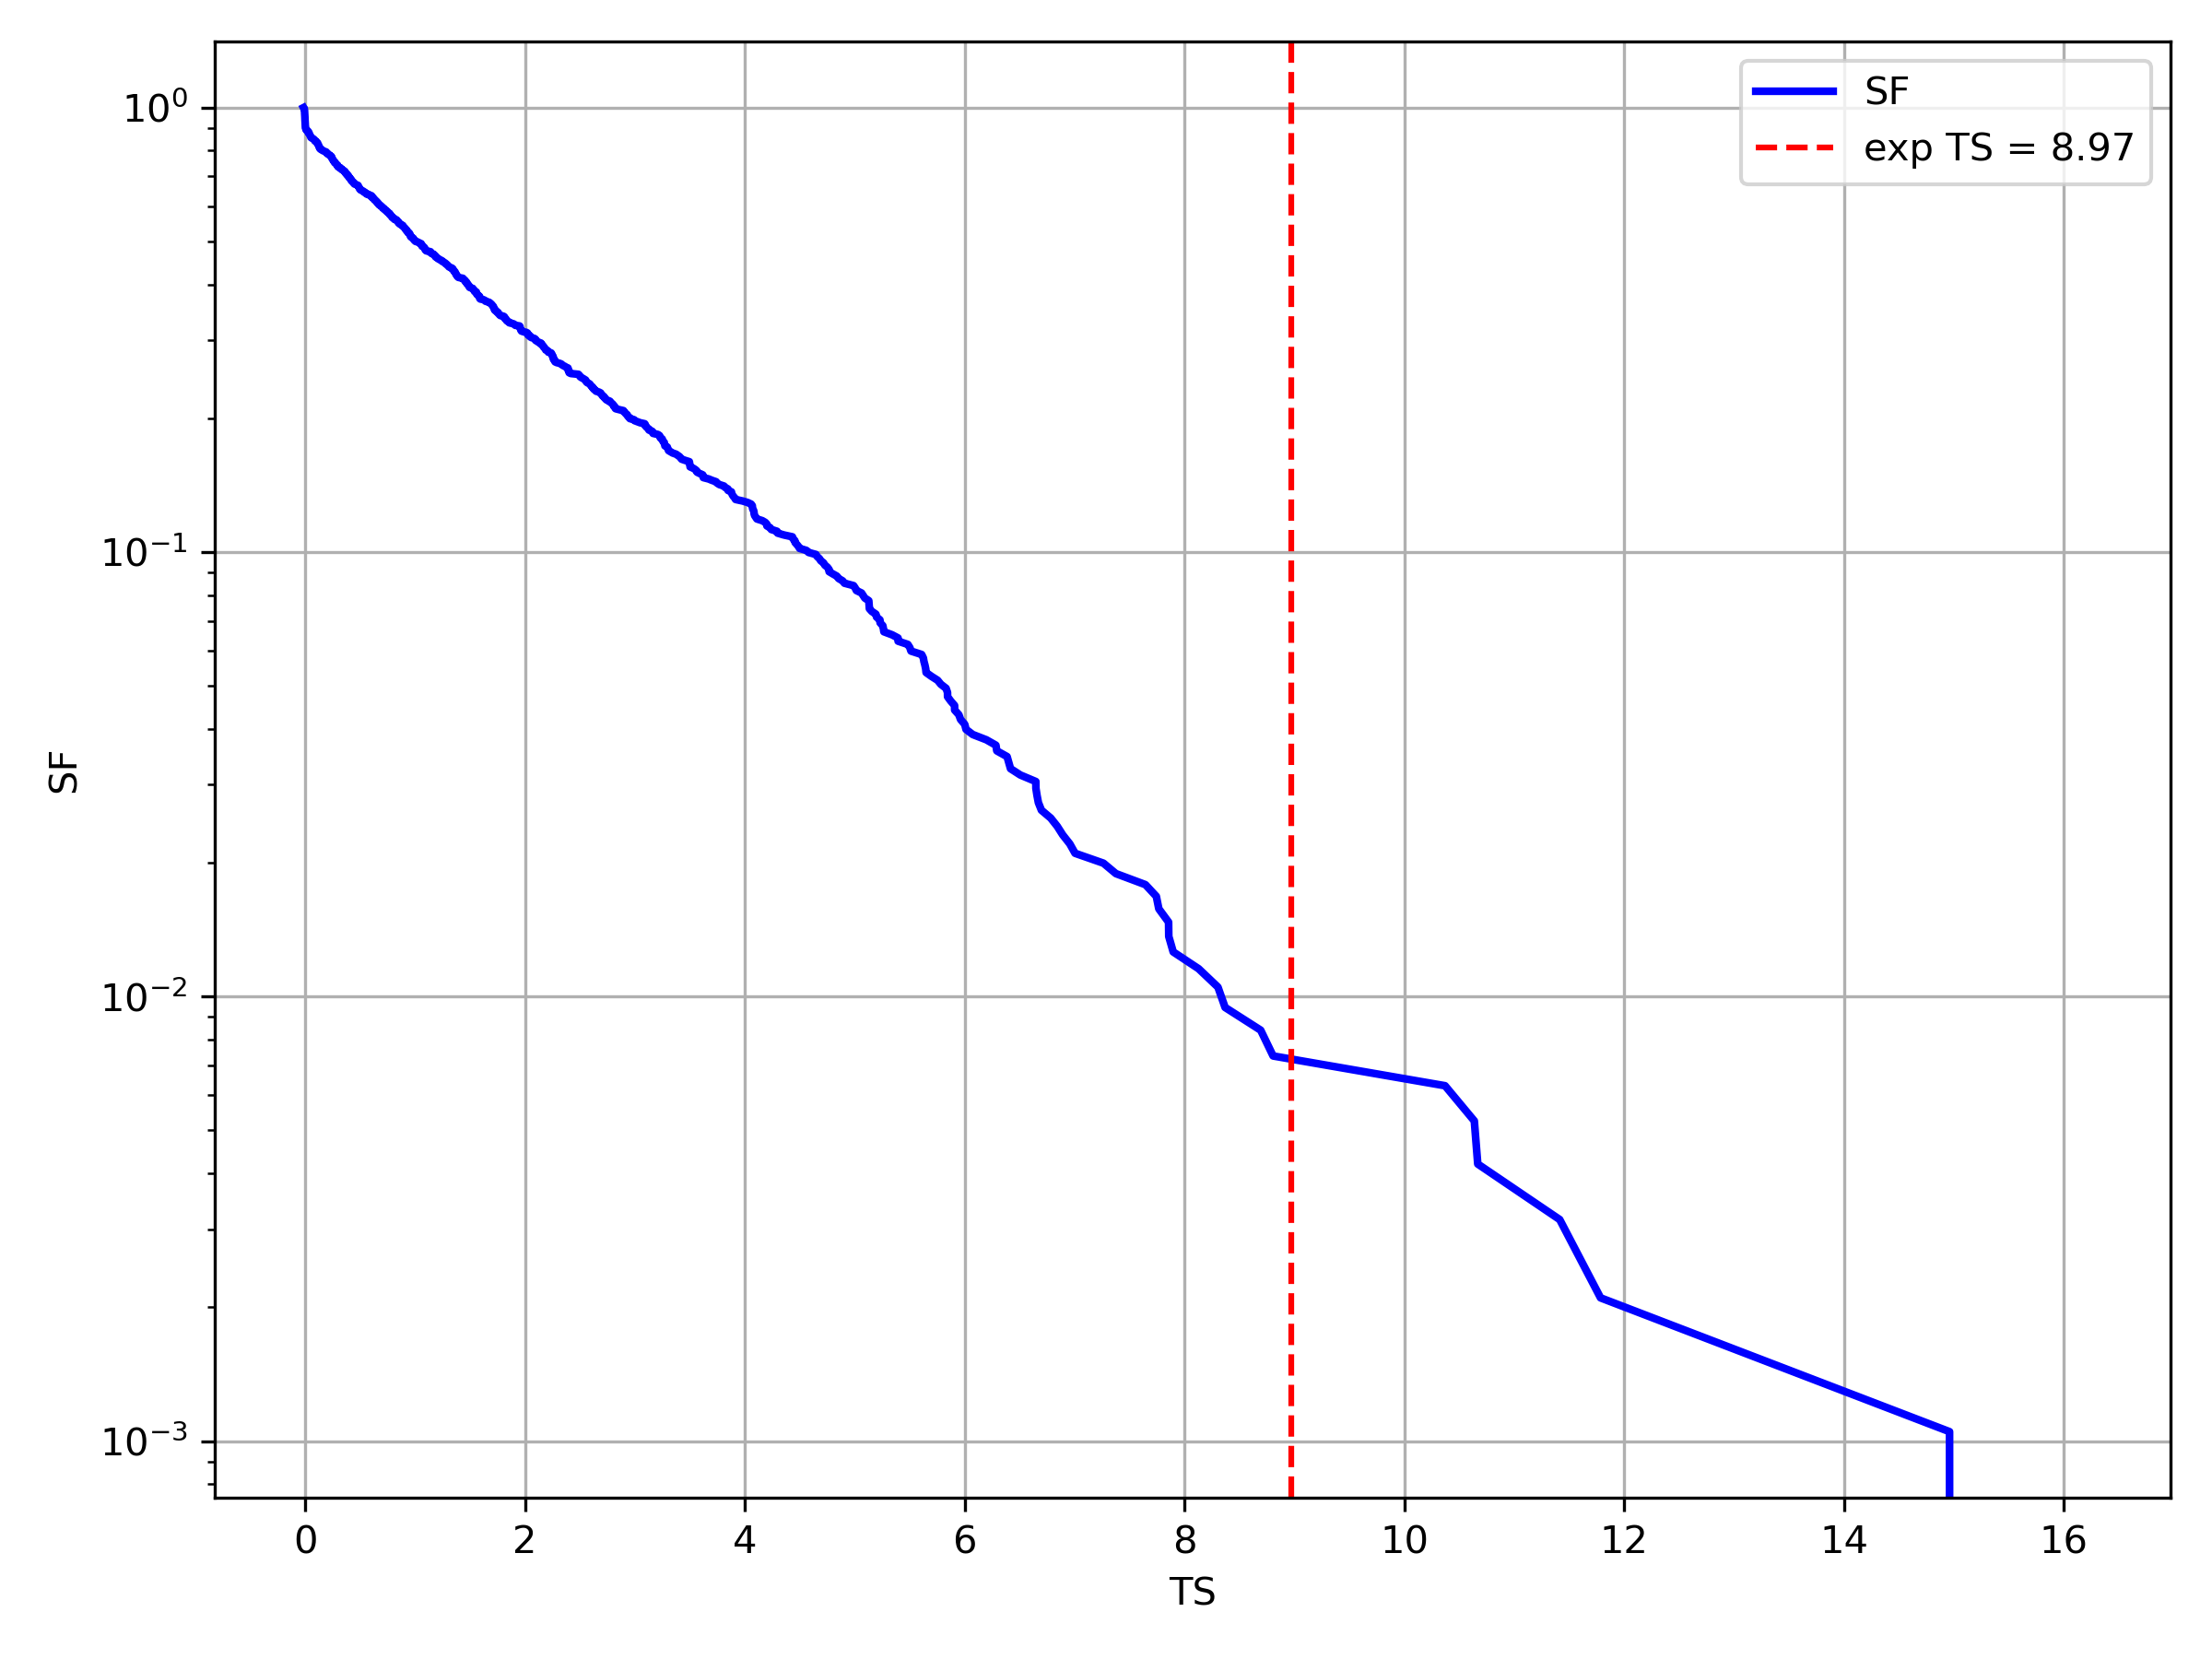
\includegraphics[width=20cm]{fig/point_source_SF.png}};
                \node[rotate=45, font=\fontsize{100}{120}\selectfont, color=gray!50, opacity=0.7] at (image1.center) {Preliminary};
            \end{tikzpicture}
            \begin{tikzpicture}
                \node[inner sep=0pt] (image2) at (0,0) {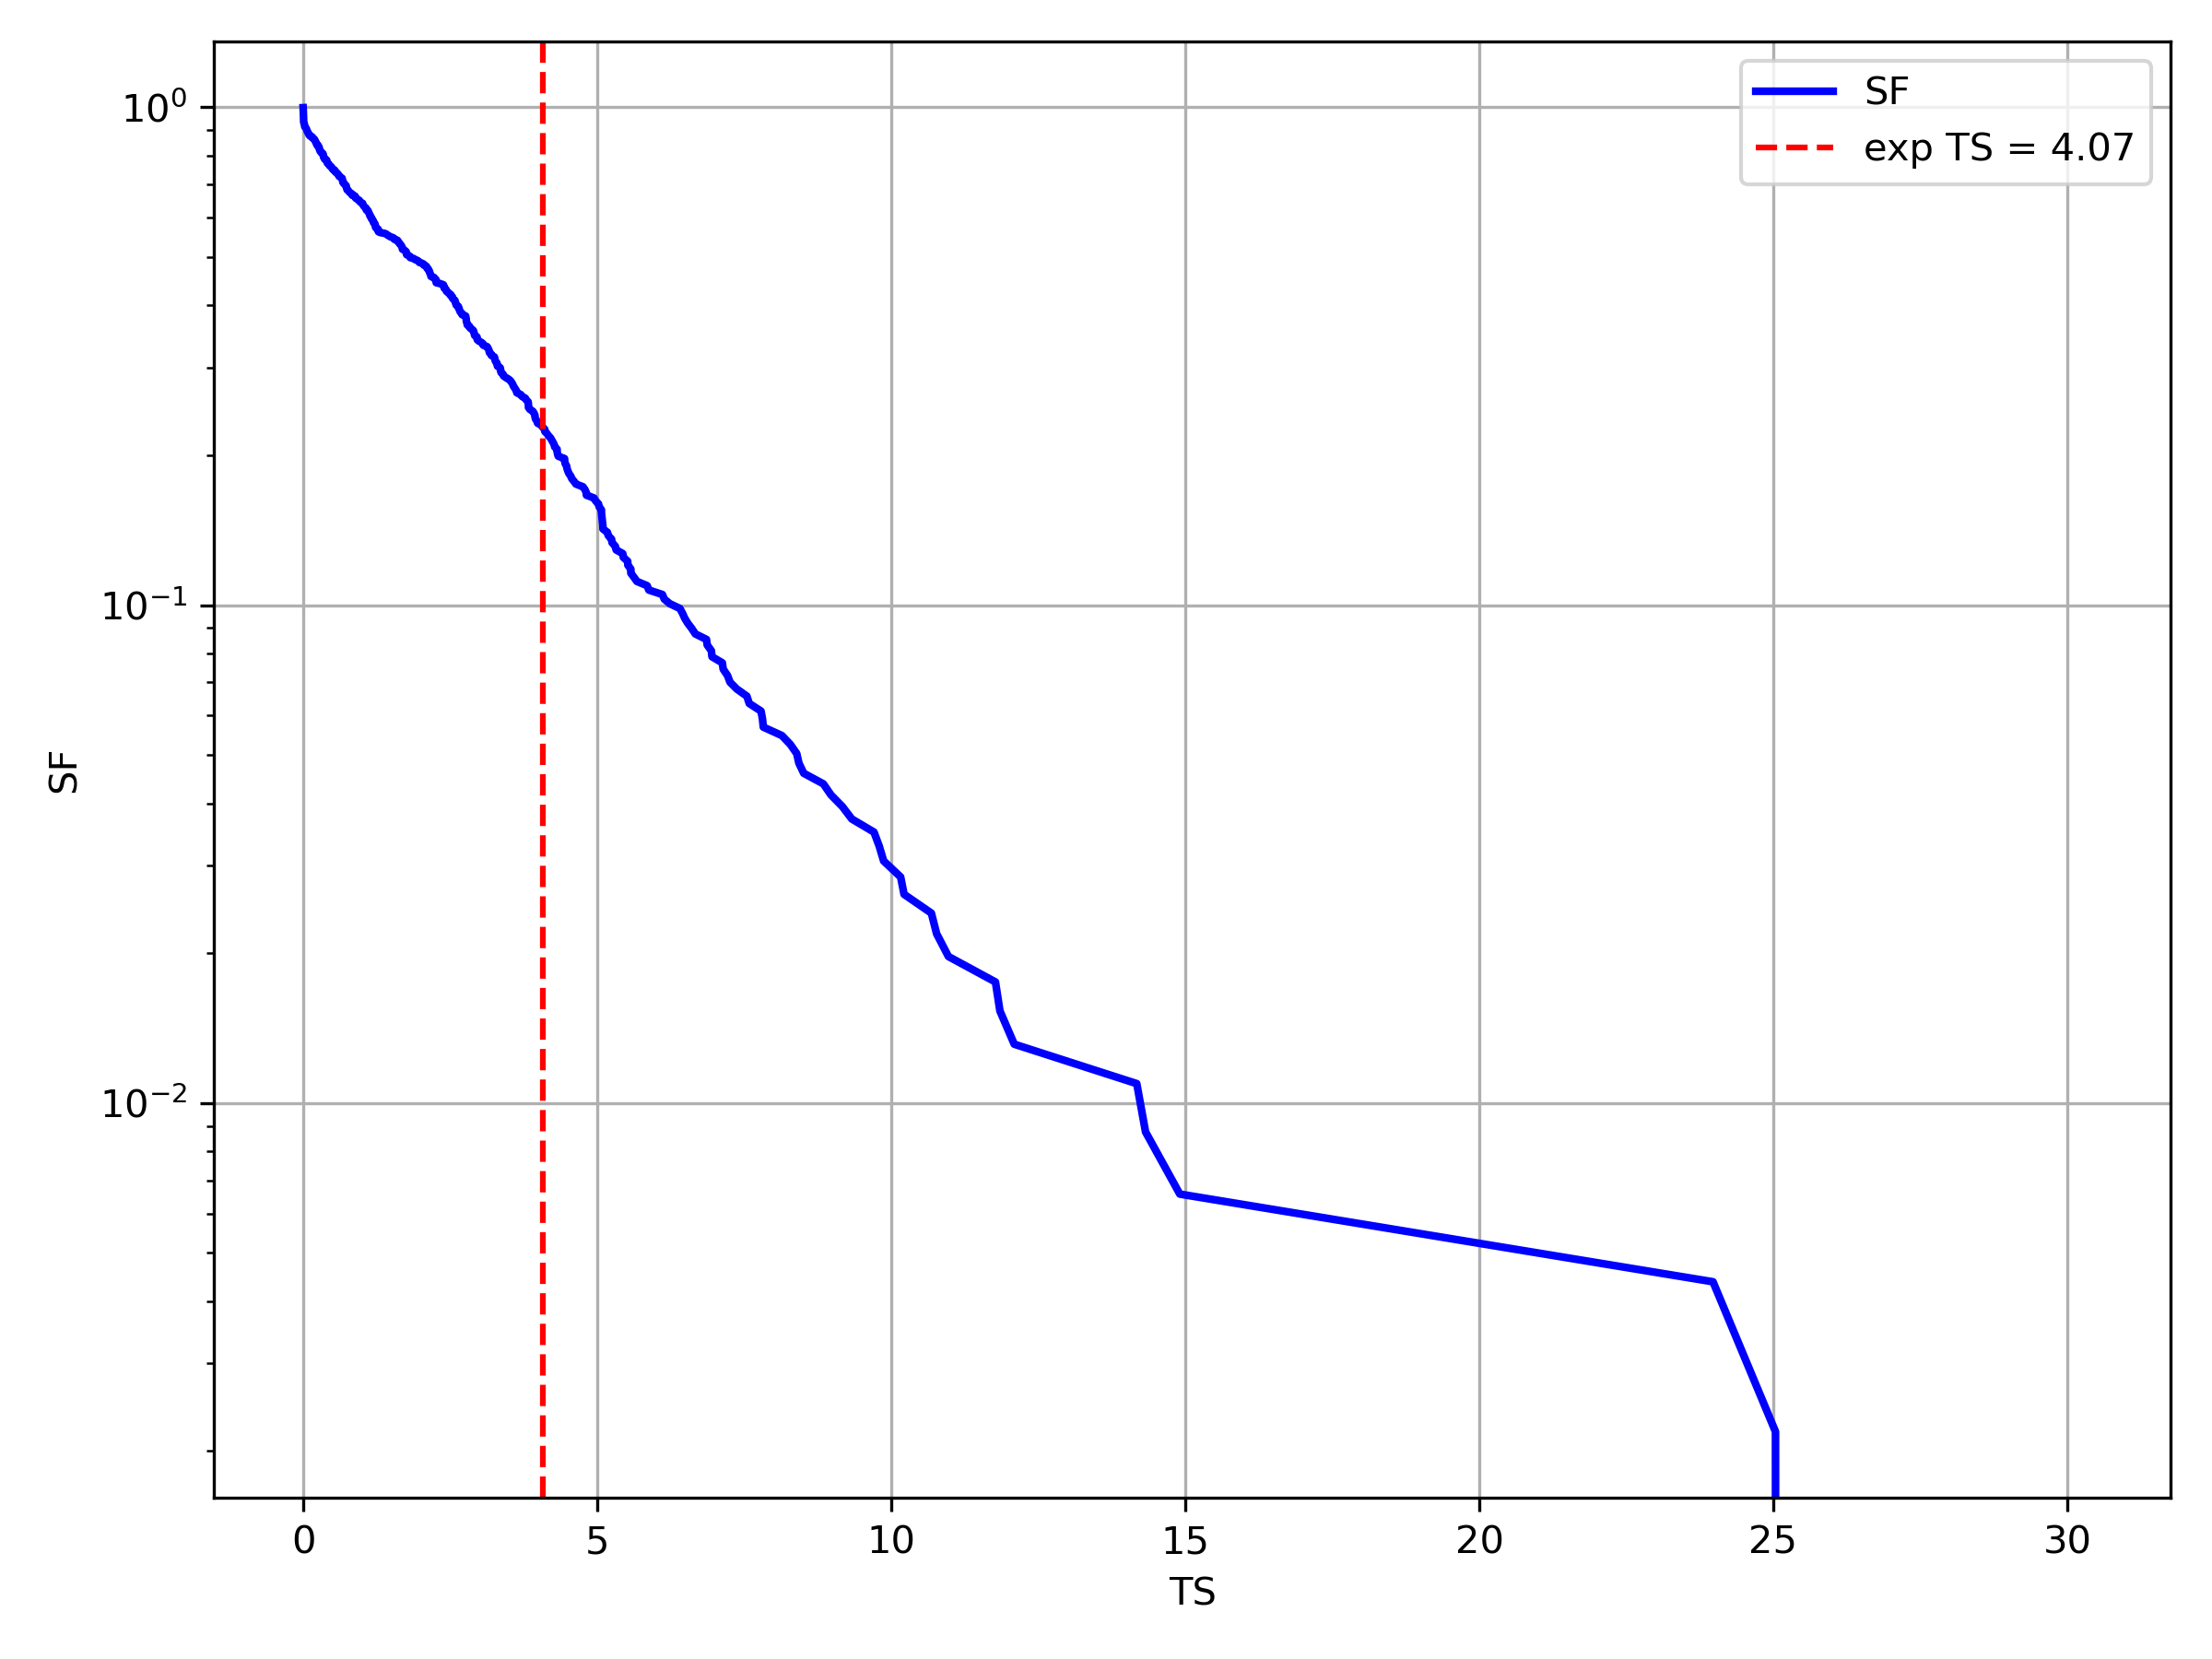
\includegraphics[width=20cm]{fig/10pc_SF.png}};
                \node[rotate=45, font=\fontsize{100}{120}\selectfont, color=gray!50, opacity=0.7] at (image2.center) {Preliminary};
            \end{tikzpicture}
        \end{minipage}

        \begin{minipage}{25cm}
                \centering 
                Figure 3: The upper and lower panels show the survival functions(SF) for the point source and extended source models, respectively. The blue lines represent the survival function of the control groups. The red dashed lines indicate the TS of the MSPs.
        \end{minipage}
        \end{center}
        
        {\LARGE Summary
        }
        \begin{itemize}[itemsep=10pt]
            % \item We investigated the potential presence of TeV halos around millisecond pulsars (MSPs) using LHAASO-WCDA data. 
            \item Analysis with point source and extended source models yields significances of 2.44$\sigma$ and 0.74$\sigma$, both below the threshold for a new discovery, indicating no detection of TeV emission or halos around MSPs.
        \end{itemize}
    }
    
\end{columns}

% %%tdli logo
% \node[anchor=south west] at (0cm,-50cm) {
\includegraphics[width=20cm]{initial_pic/tdli.png}};

% %%tdli buidling
\node[anchor=south east] at (1.cm,-59.5cm) {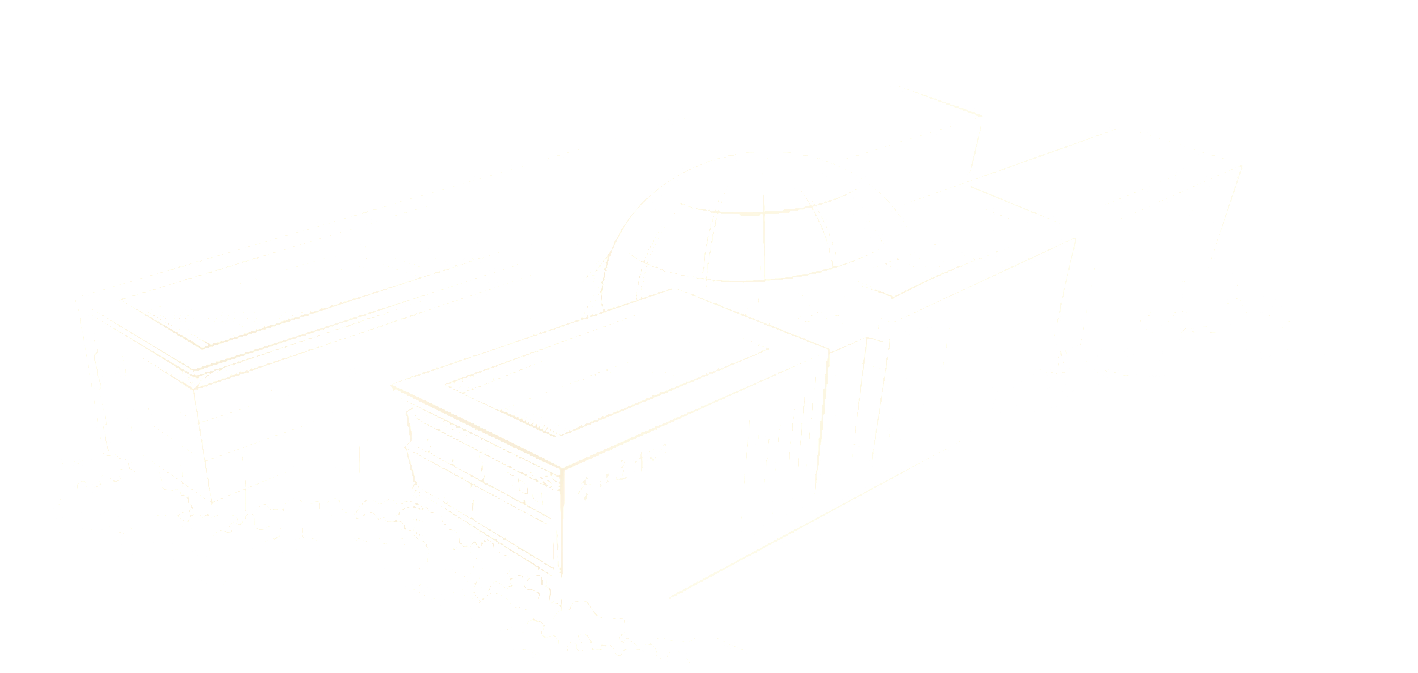
\includegraphics[width=30cm]{initial_pic/tdlibg.png}}; 

\end{document}
